\documentclass[a4paper,12pt]{article} % добавить leqno в [] для нумерации слева
\usepackage[a4paper,top=1.3cm,bottom=2cm,left=1.5cm,right=1.5cm,marginparwidth=0.75cm]{geometry}
%%% Работа с русским языком
\usepackage{cmap}					% поиск в PDF
\usepackage{mathtext} 				% русские буквы в фомулах
\usepackage[T2A]{fontenc}			% кодировка
\usepackage[utf8]{inputenc}			% кодировка исходного текста
\usepackage[english,russian]{babel}	% локализация и переносы
\usepackage{multirow}

\usepackage{graphicx}

\usepackage{wrapfig}
\usepackage{tabularx}

\usepackage{hyperref}
\usepackage[rgb]{xcolor}
\hypersetup{
colorlinks=true,urlcolor=blue
}

%%% Дополнительная работа с математикой
\usepackage{amsmath,amsfonts,amssymb,amsthm,mathtools} % AMS
\usepackage{icomma} % "Умная" запятая: $0,2$ --- число, $0, 2$ --- перечисление

%% Номера формул
\mathtoolsset{showonlyrefs=true} % Показывать номера только у тех формул, на которые есть \eqref{} в тексте.

%% Шрифты
\usepackage{euscript}	 % Шрифт Евклид
\usepackage{mathrsfs} % Красивый матшрифт

%% Свои команды
\DeclareMathOperator{\sgn}{\mathop{sgn}}

%% Перенос знаков в формулах (по Львовскому)
\newcommand*{\hm}[1]{#1\nobreak\discretionary{}
{\hbox{$\mathsurround=0pt #1$}}{}}

%% Графики
\usepackage{tikz}
\usepackage{pgfplots}
\pgfplotsset{compat=1.9}

\date{\today}

%%%%%%%%%%%%%%%%%%%%%%%%%%%%%%%%%%%%%%%%%%%%%%%%%%%%%%%%%%%%%%%%%
%%% Всё, что выше - всякие настройки для того, чтобы документ %%%
%%% компилировался и выглядел красиво. Я это никогда не       %%%
%%% трогал и тебе не советую.                                 %%%
%%%%%%%%%%%%%%%%%%%%%%%%%%%%%%%%%%%%%%%%%%%%%%%%%%%%%%%%%%%%%%%%%

\begin{document} % Начало документа

\begin{titlepage} % Далее - титульный лист
	\begin{center}
		{\large МОСКОВСКИЙ ФИЗИКО-ТЕХНИЧЕСКИЙ ИНСТИТУТ (НАЦИОНАЛЬНЫЙ ИССЛЕДОВАТЕЛЬСКИЙ УНИВЕРСИТЕТ)}
	\end{center}
	\begin{center}
		{\large Физтех-школа аэрокосмических технологий}
	\end{center}
	
	
	\vspace{4.5cm}
	{\huge
		\begin{center}
			{\bf Отчёт о выполнении лабораторной работы 2.3.1}\\
			Получение и измерение вакуума
		\end{center}
	}
	\vspace{1cm}
	\begin{center}
		{\large Соболевский Федор Александрович \\
			\vspace{0.2cm}
			Б03-109}
	\end{center}
	\vspace{8cm}
	\begin{center}
		Февраль 2022
	\end{center}
\end{titlepage} % В принципе, это стандартное оформление титульника. Что
                % за что отвечает - смотри в скомпилированном pdf.

\section{Аннотация} 

В данной работе исследовано получение вакуума различной степени разрежения с помощью механического форвакуумного и диффузионного масляного насосов. Применены различные методы измерения вакуума при давлении в диапазоне от $ 10^{-2} $ до $ 10^{-5} $ торр. С помощью основных термодинамических соотношений измерены объёмы вакуумных баллонов и скорости откачки системы в разных режимах работы. 
% С помощью $ $ можно вставлять в текст элементы формул 
% (числа в какой-то степени,
% величины таким шрифтом, какой используется в формулах, etc.)

\section{Теоретические сведения}

\subsection{Понятие вакуума}

Вакуум - пространство, свободное от вещества. В прикладной физике под вакуумом понимают среду, состоящую из газа при давлении значительно ниже атмосферного. По степени разреженности газа различают форвакуум (до $ 10^{-2} - 10^{-3}$ торр), высокий вакуум ($ 10^{-4} - 10^{-7}$ торр) и сверхвысокий вакуум ($ 10^{-8} - 10^{-11}$ торр). В данной работе исследованы способы получения и измерения форвакуума и высокого вакуума.

\subsection{Экспериментальная установка}

Установка изготовлена из стекла и состоит из форвакуумного баллона (ФБ), высоковакуумного диффузионного насоса (ВН), высоковакуумного баллона (ВБ), масляного (М) и ионизационного (И) манометров, термопарных манометров ($\text{М}_1$ и $\text{М}_2$), форвакуумного насоса (ФН) и соединительных кранов $\text{К}_1$, $\text{К}_2$, ..., $\text{К}_6$ (рис. \ref{fig:setup}). Кроме того, в состав
установки входит вариатор для регулирования тока нагревателя диффузионного насоса.
% \ref{название} - ссылка на объект с данным названием. Нумеруется автоматически.
% \eqref{название} - ссылка на уравнение/формулу. 
% Название формулы/объекта ты указываешь с помощью команды \label{название}

\begin{figure}
    \centering
    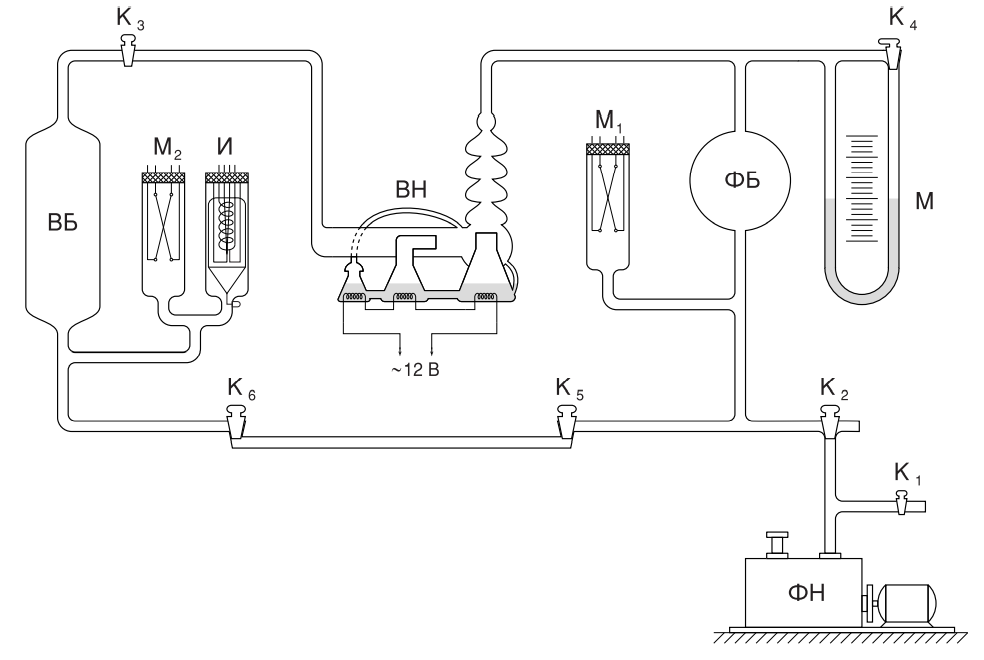
\includegraphics[width = 0.7\textwidth]{setup.PNG}
    \caption{Схема экспериментальной установки}
    \label{fig:setup}
\end{figure}
% Так вставляются изображения. Все команды довольно нехитрые.
% Изображения нужно подгружать в проект с помощью функции "Upload" в левом верхнем углу.

Трёхходовой кран $\text{К}_{2}$ используется для соединения форвакуумного насоса с установкой или атмосферой. Кран $\text{К}_3$ отделяется высоковакуумную часть установки от форвакуумной. Кран $\text{К}_4$ соединяет между собой колена манометра. Краны $\text{К}_5$ и $\text{К}_6$ стоят по концам капилляра, разделяющего форвакуумную и высоковакуумную части установки.

\begin{figure}
    \centering
    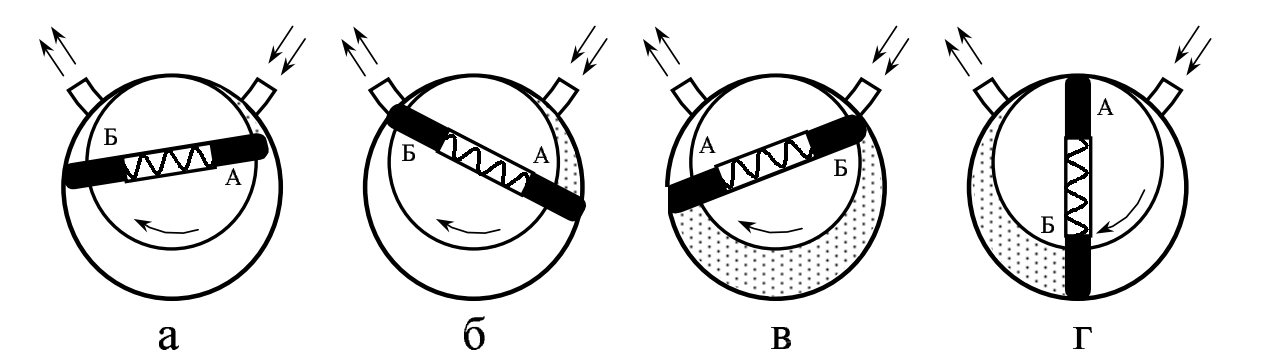
\includegraphics[width = 0.7\textwidth]{mechanic.PNG}
    \caption{Схема действия ротационного двухпластинчатого форвакуумного насоса}
    \label{fig:mechanic}
\end{figure}

Устройство и принцип действия форвакуумного насоса, используемого в данной работе, показаны на рис. \ref{fig:mechanic}. В цилиндрической полости массивного
корпуса размещен эксцентрично ротор, постоянно соприкасающийся своей верхней частью с корпусом. В диаметральный разрез ротора вставлены две пластины, раздвигаемые пружиной и плотно прижимаемые к поверхности полости. В положениях «а» и «б» пластина «А» засасывает разреженный воздух из откачиваемого объема, а пластина «Б» вытесняет ранее захваченный воздух в атмосферу. В положениях «в» и «г» пластины меняются ролями.

Откачивающее действие диффузионного насоса основано на диффузии (внедрении) молекул разреженного воздуха в струю паров масла. Попавшие в струю молекулы газа увлекаются ею и уже не возвращаются назад. На прежнем их месте образуется пустота, которая немедленно заполняется следующими порциями газа, увеличивая степень разрежения газа в окрестности струи и оказывая таким образом сильное откачивающее воздействие на весь газ в откачиваемом объеме. Скорость откачки диффузионных насосов в сотни и тысячи раз превосходит скорость откачки форвакуумного насоса.

\begin{figure}
    \centering
    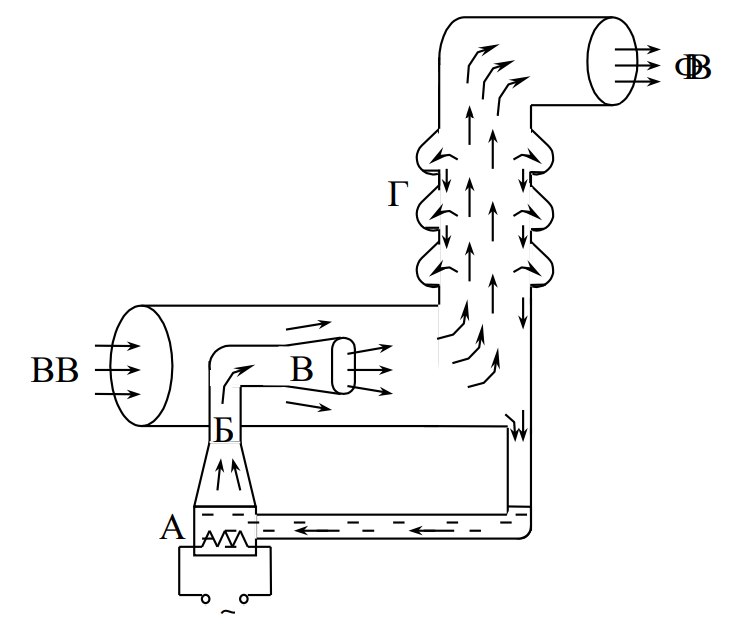
\includegraphics[width = 0.6\textwidth]{diffusion.PNG}
    \caption{Схема работы диффузионного насоса}
    \label{fig:diffusion}
\end{figure}

Устройство одной ступени масляного диффузионного насоса схематически показано на рис. \ref{fig:diffusion}. Масло, налитое в сосуд А, подогревается электрической печкой. Пары масла поднимаются по трубе Б и вырываются из сопла В. Струя паров увлекает молекулы газа, которые поступают из откачиваемого сосуда через трубку ВВ. Дальше смесь попадает в вертикальную трубу Г. Здесь масло осаждается на стенках трубы и маслосборников и стекает вниз, а оставшийся газ через трубу ФВ откачивается форвакуумным насосом.

Диффузионный насос, используемый в данном опыте, имеет две ступени и соответственно два сопла. Одно сопло вертикальное (первая ступень), второе сопло горизонтальное (вторая ступень). За второй ступенью имеется еще одна печь, пар из которой поступает не в сопло, а по тонкой трубке подводится ближе к печке первой ступени. Данная печь осуществляет фракционирование масла. Легколетучие фракции масла, испаряясь, поступают в первую ступень, обогащая ее легколетучей фракцией масла. Таким образом, первая ступень, плотность струи которой выше, начинает откачивать при более высоком давлении в форвакуумной части установки. Вторая ступень обогощается малолетучими фракциями. Плотность струи второй ступени меньше, но меньше и давление насыщенных паров масла в этой ступени. Соответственно в откачиваемый объем поступает меньше паров масла и его удается откачать до более высокого вакуума, чем при использовании одноступенчатого диффузионного насоса.

Масляный манометр М (см. рис. \ref{fig:setup}) представляет собой U-образную трубку, до половины наполненную вязким маслом, обладающим достаточно низким давлением насыщенных паров. По разности уровней масла определяется разность давлений в коленах трубки. Так как плотность масла мала, $ \rho $ = 0,9 г/$\text{см}^3$, то при помощи манометра можно измерить только небольшие разности давлений (до нескольких торр).
% Буквы греческого алфавита вставляются командами \названиеБуквы (e.g. \rho)
% Список всех символов греческого алфавита есть в документации LaTeX, просто гуглишь нужный символ и переходишь по первой ссылке.

\begin{figure}
    \centering
    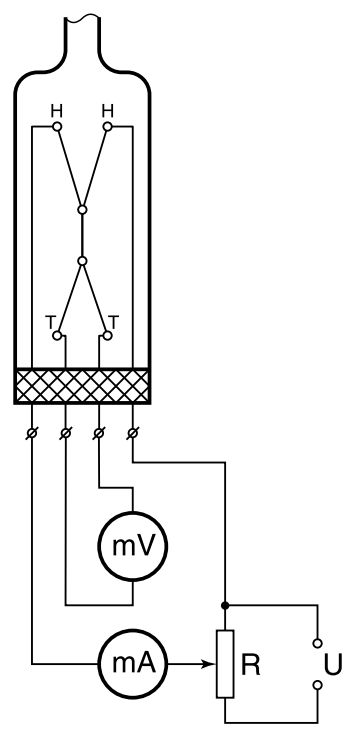
\includegraphics[width = 0.3\textwidth]{thermo.PNG}
    \caption{Схема устройства термопарного манометра ПМТ-2}
    \label{fig:thermo}
\end{figure}

Чувствительным элементом термопарного манометра является платино-платинородиевая термопара, спаянная с никелевой нитью накала и заключенная в стеклянный баллон (лампа ПМТ-2). Устройство термопары показано на рис. \ref{fig:thermo}. По нити накала НН пропускается ток постоянной величины. Для установки тока служит потенциометр R. Термопара ТТ присоединяется к милливольтметру, показания которого определяются температурой нити накала и зависят от отдачи тепла в окружающее пространство. Потери тепла определяются теплопроводностью нити и термопары, теплопроводностью газа, переносом тепла конвективными потоками газа внутри лампы и теплоизлучением нити (инфракрасное тепловое излучение). В обычном режиме лампы основную роль играет теплопроводность газа. При давлениях > 1 торр теплопроводность газа, а вместе с ней и ЭДС термопары практически не зависят от давления газа, и прибор не работает.

При улучшении вакуума средняя длина свободного пробега молекул становится сравнимой с диаметром нити, теплоотвод падает и температура спая возрастает. При вакууме ~$10^{-3}$ торр теплоотвод, осуществляемый газом, становится сравнимым с другими видами потерь тепла и температура нити становится практически постоянной. На рис. \ref{fig:grad} приведена градуировочная кривая термопары ПМТ-2.

\begin{figure}
    \centering
    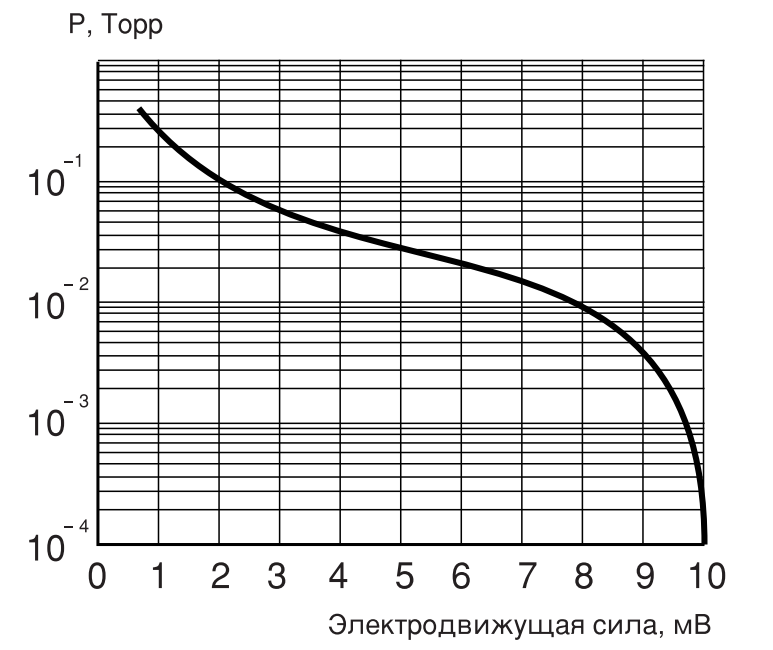
\includegraphics[width = 0.5\textwidth]{grad.PNG}
    \caption{Градуировочная кривая термопары ПМТ-2}
    \label{fig:grad}
\end{figure}

\begin{figure}
    \centering
    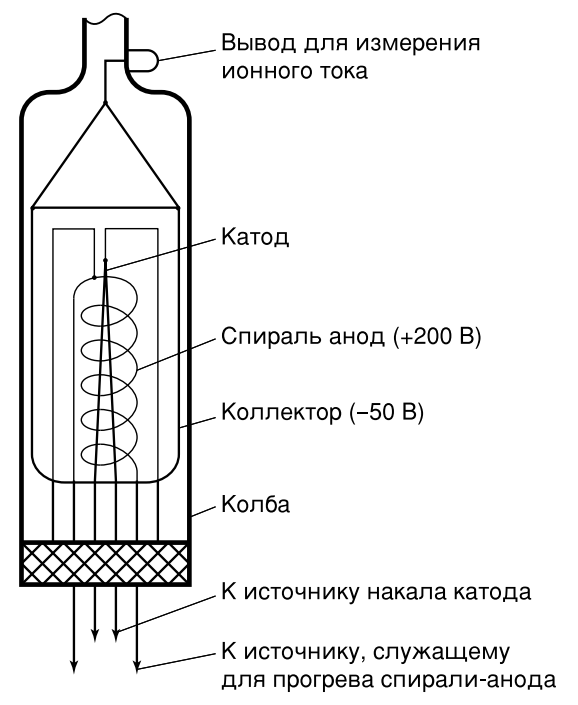
\includegraphics[width = 0.35\textwidth]{ion.PNG}
    \caption{Схема ионизационной лампы ЛМ-2}
    \label{fig:ion}
\end{figure}

Ионизационный манометр представляет собой трёхэлектродную лампу (см. рис. \ref{fig:ion}). Электроны испускаются катодом и увлекаются электрическим полем к аноду, имеющему вид редкой спирали, за витки которой электроны проскакивают и, замедляясь полем коллектора, возвращаются назад. Прежде чем осесть на аноде, электроны многократно пересекаются пространство между катодом и коллектором, ионизируя частицы газа на своём пути. Ионы притягиваются полем коллектора и определяют его ток, который оказывается пропорциональным плотности газа и, следовательно, может служить мерой давления. Калибровка манометра верна, если остаточным газом в колбе является воздух. При давлении выше $10^{-3}$ катод манометра перегорает, поэтому данный прибор применим только для измерения очень малых величин давления.

\subsection{Процесс откачки}

Мерой производительности насоса является скорость откачки $W$: $[W] = 1 $ л/с - объём газа, удаляемого из сосуда за единицу времени. Скорость откачки форвакуумного насоса можно считать равной объёму воздухозаборной камеры, умноженному на число оборотов в секунду.
% Обычно при работе с математическими символами внутри текста следует аккуратно расставлять между ними пробелы, чтобы выглядело красиво. Пробелы внутри уравнения не отображаются. Также стоит обратить внимание, что большие математические выражения по типу дробей в показателе степени, операторов суммирования с индексами и т.п. будут очень неаккуратно выглядеть внутри текста, поэтому их лучше выносить или записывать более "строчно".
% Русский текст внутри уравнения отображаться не будет, поэтому для того, чтобы поставить в индекс русскую букву или возвести сантиметры в квадрат, используй команду \text{текст}.

Рассмотрим обычную схему откачки. Обозначим величины, характеризующие поступление газа обратно в систему в единицу времени: $Q_1$ - количество газа, десорбирующегося с поверхности откачиваемого объёма, $Q_2$ - количество газа, проникающего в объём извне - через течи, $Q_3$ - количество газа, поступающего из насоса назад в систему. Количества газа $Q_1$, $Q_2$, $Q_3$ можно измерять в единицах $PV$ с точностью до множителя $RT$. Основное уравнение, описывающее процесс откачки:

\begin{equation}
    -VdP = (PW - Q_1 - Q_2 - Q_3)dt.
    \label{pumpout}
\end{equation}
% Вот уравнение. Если в тексте есть ссылка на уравнение по его label, то оно автоматически нумеруется справа.
% На всякий случай: нижние индексы делаются с помощью _ после символа, верхние - с помощью ^ . Если нужно поставить несколько символов в индекс, используй фигурные скобки: Q_{Q_Q}.

При достижении предельного вакуума с давлением $P_\text{пр}$ $\frac{dP}{dt} = 0$, поэтому уравнение \eqref{pumpout} принимает вид

\begin{equation}
    P_\text{пр}W = \sum\limits_i Q_i.
    \label{pumpoutLimit}
\end{equation}
% Все математические символы, кроме базовых, задаются в LaTeX командами через \. Посмотреть полный список символов можно, опять же, в документации.

Обычно $Q_i$ слабо зависят от времени, поэтому их, как и $W$, можно считать постоянными. Интегрируя с учётом этого \eqref{pumpout} и применяя \eqref{pumpoutLimit}, можно получить

\begin{equation}
    P - P_\text{пр} = (P_0 - P_\text{пр})e^{-\frac{W}{V}t},
    \label{pressure1}
\end{equation}

где $P_0$ - начальное давление. Так как $P_\text{пр}$ велико по сравнению с $P_0$, можно записать, что

\begin{equation}
    P = P_0e^{-\frac{W}{V}t}
\end{equation}

Следует иметь в виду, что реальная вакуумная система состоит, помимо насоса, из множества других элементов, имеющих свом пропускные способности $C_i$. При этом полная скорость откачки $W$ и собственная скорость откачки насоса $W_H$ при этом связаны соотношением 

\begin{equation}
    \frac{1}{W} = \frac{1}{W_H} + \sum\limits_i C_i.
\end{equation}

\subsection{Течение газа через трубу}

Характер течения газа существенно зависит от соотношения между размерами системы и длиной свободного пробега молекул. При нормальном атмосферном давлении и даже при достижении форвакуума длина свободного пробега молекул меньше диаметра трубок и течение откачиваемого газа определяется его вязкостью (взаимодействием молекул). При переходе к высокому вакууму соударения молекул между собой начинают играть меньшую роль, чем взаимодействие со стенками сосуда. Для течения газа через трубу кругового сечения в условиях высокого вакуума (в кнудсеновском режиме), справедлива формула

\begin{equation}
    \frac{d(PV)}{dt} = \frac{4}{3}r^3\sqrt{\frac{2\pi RT}{\mu}}\frac{P_2 - P_1}{L}.
    \label{throughput}
\end{equation}

Пренебрегая давлением $P_1$ у конца, обращённого к насосу, получим выражение для пропускной способности трубы

\begin{equation}
    C_\text{тр} = (\frac{dV}{dt})_\text{тр} = \frac{4}{3}\frac{r^3}{L}\sqrt{\frac{2\pi RT}{\mu}}.
\end{equation}

\section{Оборудование и экспериментальные погрешности}

\textbf{В работе использовались:} вакуумная установка с высоковакуумным и форвакуумным баллонами, форвакуумным и диффузионным насосами, двумя термопарными, ионизационным и масляным манометрами и вариатором для регулирования тока, секундомер. 
% Команды \textbf{текст}, \textit{текст} отвечают за жирный шрифт и курсив соответственно.

\textbf{Инструментальные погрешности:}

\begin{itemize}
    \item \textbf{Масляный манометр:} $\Delta_\text{мм} = 0,5$ мм,
    \item \textbf{Секундомер:} $\Delta_\text{с} = 0,01 $ с.
\end{itemize}
% Обрати внимание: вид символа может зависеть от того, заглавная или строчная буква в начале (например, \delta и \Delta).

\section{Результаты измерений и обработка экспериментальных данных}

\subsection{Измерение объёмов форвакуумной и высоковакуумной частей установки}

Для измерения объёмов форвакуумной и высоковакуумной частей экспериментальной установки между кранами $\text{К}_5$ и $\text{К}_6$ был заперт известный объём ($V_0 = 50 \text{ см}^2$) воздуха при нормальном атмосферном давлении ($P_\text{атм} = 1 $ атм). Затем установка была откачана до форвакуума, после чего запертый между кранами воздух был выпущен поочерёдно в форвакуумную и высоковакуумную части установки. Давление в установке было измерено с помощью масляного манометра: его можно определить по формуле

\begin{equation}
    P = \rho_\text{м} g\Delta h,
    \label{oilManometer}
\end{equation}

где $\rho_\text{м} = 0,885 \frac{\text{г}}{\text{см}^3}$ - плотность масла в манометре, $\Delta h$ - разница высот между коленами манометра. Так как температура в установке поддерживается примерно постоянной, а давление форвакуума в установке пренебрежимо мало по сравнению с давлением запертого газа, то, зная начальный объём и давление, можно из полученного значения давления определить объём частей установки, используя закон Бойля-Мариотта об изотермическом расширении газа:

\begin{equation}
    T = \text{const} \iff PV = \text{const}.
    \label{Boyle-Mariotte}
\end{equation}

Используя соотношения \eqref{oilManometer} и \eqref{Boyle-Mariotte}, для объёмов $V_\text{фв}$ форвакуумной и $V_\text{вв}$ высоковакуумной частей установки получаем

\begin{equation}
    V_\text{фв} = \frac{P_\text{атм}V_0}{\rho_\text{м}g\Delta h_\text{фв}} - V_0,
\end{equation}
    
\begin{equation}
    V_\text{вв} = \frac{P_\text{атм}V_0}{\rho_\text{м}g\Delta h_\text{вв}} - V_0 - V_\text{фв}.
\end{equation}

Измерения для данного опыта были проведены два раза. Полученные значения представлены в таблице \ref{tab:volumes}. Как видно из результатов вычислений, значения различаются между собой из-за неточности данного метода. Для последующих измерений было взято среднее значение объёма высоковакуумной части установки: 

\begin{itemize}
    \item $V = 1223,3 \text{ см}^3 \approx 1,223 \text{ л}$.
\end{itemize}

\begin{table}[] % А вот и таблица подъехала. 
    \centering
    \begin{tabular}{|c|c|c|c|c|c|c|c|c|} \hline % В этой строчке с помощью |c|...|c| указывается количество столбцов и наличие разделителей между ними.
    % \hline - указатель на горизональную черту НАД данной строкой. 
        № опыта & h_1^\text{фв}, \text{мм} & h_2^\text{фв}, \text{мм} & \Delta h_\text{фв}, \text{мм} & V_\text{фв}, \text{см}^3 & h_1^\text{вв}, \text{мм} & h_2^\text{вв}, \text{мм} & \Delta h_\text{вв}, \text{мм} & V_\text{вв}, \text{см}^3\\ \hline % Таблицы в LaTeX пишутся в строчку. К сожалению. Разделяются ячейчки знаком &. Конец строки обозначается \\.
        1 & 34,2 & 9,0 & 25,2 & 2310,7 & 30,0 & 14,0 & 16,0 & 1331,5 \\ \hline
        2 & 34,3 & 8,9 & 25,4 & 2292,4 & 31,0 & 13,9 & 17,1 & 1115,1 \\ \hline
    \end{tabular}
    \caption{Результаты измерения объёмов форвакуумной и высоковакуумной частей установки}
    \label{tab:volumes}
\end{table}
% На таблицы, как и на рисунки, можно делать ссылки по \ref{}. Нумеруются они также автоматически.

\subsection{Получение высокого вакуума и измерение скорости откачки}

Во второй части экспериментальной работы в высоковакуумной части установки с помощью диффузионного насоса был получен вакуум с предельным давлением $P_\text{пр} = 1,0 \cdot 10^{-4} $ торр. Затем вакуум был ухудшен путём перекрытия крана, соединяющего насос и высоковакуумный баллон, а после снова улучшен. При этом получена зависимость давления в системе от времени при улучшении вакуума, изображенная на рис. \ref{graph}. 

% Не уверен, что тебе захочется мучиться с графиками в LaTeX, но на всякий случай поясню этот ужас.
\begin{figure} % График - тоже рисунок.
\centering
\resizebox {0.85\textwidth} {!} {
\begin{tikzpicture} % Объявление графика PGFPlots.
\begin{axis}[ ylabel = {$ \ln{\frac{P - P_\text{пр}}{P_0 - P_\text{пр}}} $}, xlabel = {$ t $, с}, xmin = 0, xmax = 12, ymin = -4.2, ymax = 0, legend style={legend style={at={(axis cs:12, 0)},anchor=north east}}] % Здесь много всего. Сначала под ylabel и xlabel в фигурных скобках идут подписи осей, далее xmin, xmax и ymin, ymax - минимальные/максимальные значения осей. Команду, отвечающую за легенду, не трогай, умоляю - я с ней в своё время отмучился полдня. После axis cs: пишутся через запятую координаты легенды, после anchor= - расположение якоря (какая именно точка легенды лежит на заданных тобою координатах).  

\addplot[color=black, mark=x, only marks] coordinates{(0.51, -0.07)(1, -0.14)(1.5, -0.22)(2.02, -0.33)(2.52, -0.5)(3.08, -0.68)(3.43, -0.85)(3.98, -1.07)(4.48, -1.34)(5, -1.55)(5.51, -1.81)(6, -2.03)(6.48, -2.16)(6.96, -2.32)(7.47, -2.5)(8, -2.72)(8.5, -3.01)(9.53, -3.42)(11.01, -4.11)}; % Добавление графика. color= - цвет, mark= - вид точки (можно попробовать поискать все возможные виды в документации, я знаю только o, x, *, square и triangle. Можно не писать mark=, тогда будут просто точки), only marks - флажок, означающий отсутствие соединяющей отметки линии. Далее в команде coordinates{} указываются поочерёдно координаты точек на графике. Они указываются в скобках через запятую (десятичные дроби пишем через точку), между скобками ничего не ставится.
% ВАЖНО: PGFPlots - штука весьма деликатная, поэтому при неправильном синтаксисе не скомпилируется вообще ничего. Это стоило мне половины моих нервных клеток. Если вдруг не скомпилировалось - проверяй, там ли у тебя стоят запятые, не написала ли ты через запятую десятичную дробь, не забыла ли ты точку с запятой после строчки с \addplot и т.п. Обычно компилятор в таком случае просто пишет без объяснений "Runaway argument?".

\addplot[color=black, mark=o, only marks] coordinates{(0.47, -0.03)(0.88, -0.11)(1.38, -0.18)(1.87, -0.33)(2.38, -0.43)(2.87, -0.66)(3.38, -0.8)(3.86, -1)(4.36, -1.26)(4.87, -1.53)(5.36, -1.79)(5.85, -2.01)(6.36, -2.15)(6.85, -2.48)(7.37, -2.71)(8.4, -3)(9.39, -3.4)(11.44, -4.09)};
\legend{Опыт № 1, Опыт № 2} % Легенда для тех графиков, что сверху. Через запятую указываются подписи графиков по очереди.
\addplot[color=blue] coordinates{(0, 0)(12, -4.044)}; % Здесь я построил прямые с помощью двух точек. Почему не с помощью y = kx + b? PGFPlots позволяет строить графики с помощью уравнений по типу y = x^2 - 2, но он это делает только в диапазоне от 0 до 5 или что-то около. Почему - god knows.
\addplot[color=red] coordinates{(0, 0)(12, -4.104)};

\end{axis}
\end{tikzpicture}
}
\caption{Зависимость падения давления от времени при улучшении вакуума}
\label{graph}
\end{figure}
% Если вдруг будешь пользоваться, настоятельно рекомендую не трогать синтаксис, который я здесь подогнал. Ломается всё на раз-два.
% Ну и, конечно, есть вариант для умных - пользоваться графиками в Python. Я пока до этого не дорос.

Из \eqref{pressure1} зависимость $ \ln{\frac{P - P_\text{пр}}{P_0 - P_\text{пр}}} $ от времени линейна:

\begin{equation}
    \ln{\frac{P - P_\text{пр}}{P_0 - P_\text{пр}}} = -\frac{W}{V}t,
\end{equation}

где $ V = V_\text{вв}$, $-\frac{W}{V}$ - коэффициент наклона прямой. С помощью метода наименьших квадратов найдены следующие значения данного коэффициента и соответствующие им величины скорости откачки системы:

\begin{itemize}
    \item Опыт № 1: $-\frac{W}{V} = -0,337 \text{ с}^{-1}$, $W = 0,276 $ л/с;
    \item Опыт № 2: $-\frac{W}{V} = -0,342 \text{ с}^{-1}$, $W = 0,280 $ л/с.
\end{itemize}
% Ещё одна полезная штука - itemize и enumerate. itemize делает список с маркерами в виде точек, enumerate - пронумерованный список. Каждый новый элемент начинается с \item.

Пользуясь полученными значениями, можно оценить сумму всех натеканий $\sum\limits_i Q_i$ в систему:

\begin{equation}
    \sum\limits_i Q_i = P_\text{пр}W = 3,7 \text{ мДж/с}.
\end{equation}

Скорость откачки также можно вычислить в стационарном режиме, зная предельное давление и установившееся давление при наличии искусственной щели. Для этого было измерено давление, установившееся после открытия капилляра между кранами $\text{К}_5$ и $\text{К}_6$. Установившееся давление $P_\text{уст}$ и $P_\text{пр}$ связаны соотношениями

\begin{equation}
    P_\text{пр}W = \sum\limits_i Q_i, \;\;\;\;\; % Так я пытался вставить пробел между двумя уравнениями в одном.
    P_\text{уст}W = \sum\limits_i Q_i + \frac{d(PV)}{dt}
\end{equation}

Подстановкой первого выражения во второе с использованием \eqref{throughput} получено общее уравнение

\begin{equation}
    (P_\text{уст} - P_\text{пр})W = \frac{4}{3}r^3\sqrt{\frac{2\pi RT}{\mu}}\frac{P_\text{уст}}{L}.
    \label{equatio}
\end{equation}

При открытии капилляра длины $L = 10,8$ см и радиуса $r = 0,4$ мм, соединяющего высоковакуумную и форвакуумную части установки, установилось давление $P_\text{уст} = 1,5 \cdot 10^{-4}$ торр. Из уравнения \eqref{equatio} получено следующее значение скорости откачки $W$:

\begin{itemize}
    \item $W = 0,260 $ л/с.
\end{itemize}

\section{Обсуждение результатов и вывод}

В данном работе были рассмотрены и проверены методы получения и измерения вакуума различной степени разрежения. Опыт показал, что для работы с различными по порядку величины значениями давления требуются приборы различной точности и что более точные приборы оказываются более чувствительными. 

Погрешность полученных результатов, однако, остаётся значительной. Ошибка измерений особенно заметна в значениях объёмов, которые различаются почти на 10\%. Данные неточности могли возникнуть из-за непостоянства температуры и неквазистатичности исследуемых процессов. Из-за большой ошибки косвенных измерений предпочтительнее использовать точные значения объёмов, указанные производителем установки. 
Неточности в измерении скорости откачки системы могли возникнуть из-за неучтённых значений пропускных способностей отверстий в системе, параметры которых не были указаны на установке. Также при определении линейного коэффициента в зависимости давления от времени было неучтено постепенное изменение пропускной способности крана при его постепенном отвинчивании.

Несмотря на погрешности измерений, исследованные в работе известные характерные свойства низкого и высокого вакуума подтвердились на практике, и способы его измерения оказались применимы. Для получения вакуума со степенью разрежения меньше $1,0 \cdot 10^{-4}$ следует использовать другие приборы и методы, например, комбинированную откачку.  

\end{document}

% Всё! Надеюсь, сильно больше, чем тут уже есть, тебе в отчётах не понадобится. Если что - смотри документацию LaTeX.
